
在我们已经了解过的顺序数据结构中,数据都存储在一个数组中(或者是一个由内存块组成的数组)。现在我们将考虑一种不同类型的数据结构,其中数据是通过指针连接在一起的。最简单的例子就是一个链表,其中每个元素都是单独分配的,这里了解到的方法也适用于其他节点容器,如树、图或其他数据结构,其中每个元素都是单独分配的,数据通过指针连接在一起。

为了简单起见,我们先来看一个单链表。在STL中,为\texttt{std::forward\_list}:

%\hspace*{\fill} \\ %插入空行
\begin{center}
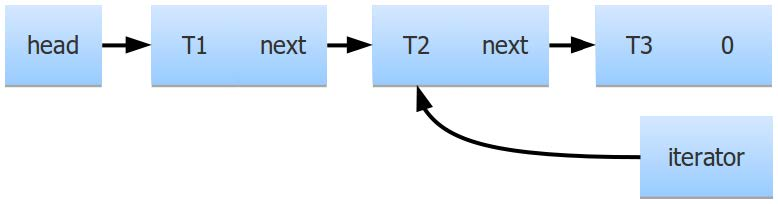
\includegraphics[width=0.9\textwidth]{content/2/chapter7/images/24.jpg}\\
图7.24 - 带有迭代器的单链表
\end{center}

因为每个元素都是单独分配的,所以也可以单独回收。通常,轻量级分配器用于这些数据结构,其中内存在大块中分配,这些大块划分为节点大小的片段。当一个节点释放时,内存不会返回给操作系统,而是放在一个空闲列表中,以便应对下一次分配内存的请求。就我们的目的而言,内存直接从操作系统分配,还由专门的分配器处理,与我们的关系不大(后者通常更高效)。

并发程序中,链表的迭代器是一个挑战。如图7.24,这些迭代器可以指向链表中的任何位置。如果有元素从列表中删除,则希望它的内存能够用于构造和插入另一个元素(如果不这样做,并保持所有内存直到整个列表删除,重复增加和删除元素会浪费大量的内存)。但是,如果有指向链表节点的迭代器,则不能删除该节点。在单线程程序中也是如此,但是在并发程序中的管理通常要困难得多。对于可能使用多个线程的迭代器,通常不能通过操作的执行流保证没有迭代器指向要删除的元素。本例中,需要迭代器来扩展它们所指向的链表节点的生命周期。当然,这是一个使用引用计数的智能指针的工作,比如\texttt{std::shared\_ptr}。现在,我们假设链表中的所有指针,包括连接节点和迭代器中的指针,都是智能指针(\texttt{std::shared\_ptr}或类似的具有强线程安全保证的指针)。

就像处理顺序数据结构一样,对线程安全的数据结构的第一次尝试应该是使用锁保护的实现。在确定需要之前,永远不要设计无锁数据结构:开发无锁代码可能很酷,但试图在其中找到bug则很困难。

就像前做的那样,我们必须重新设计部分接口,所有的操作都是事务性的:例如,\texttt{pop\_front()}应该工作,无论链表是否为空。然后,可以用锁保护所有操作。对于\texttt{push\_front()}和\texttt{pop\_front()}这样的操作,很可能类似于之前观察到的堆栈或队列的性能。这份清单还列出了我们此前没有面过的挑战。

首先,该链表支持在任意位置插入。对于\texttt{std::forward\_list},在迭代器指向的元素之后插入一个新元素可以使用\texttt{inser\_after()}。若同时在两个线程上插入两个元素,我们希望插入操作可以并发进行,除非这两个位置非常接近,并且影响相同的链表节点。但是,我们不能用一个锁来保护整个链表。

如果考虑长时间运行的操作,比如在列表中搜索具有所需值(或满足其他条件)的元素,情况会更糟。整个搜索操作中,必须锁定列表,因此在遍历列表时不能向列表添加或删除元素。当然,如果经常进行搜索,链表不是合适的数据结构,但树和其他节点数据结构也有相同的问题:如果需要遍历数据结构的大部分,需要在整个操作期间持有锁,从而阻塞所有其他线程访问,甚至与我们当前操作无关的节点上的操作也会阻塞。

当然,如果从未遇到过这些问题,那么就不必担心这些问题:如果链表仅从前端和后端访问,那么用一个锁保护的列表可能就足够了。在设计并发数据结构时,不必要的通用性是头痛的关键。不过这里,只需要构建需要的内容即可。

然而,大多数时候,节点数据结构并不仅仅是从端点访问的,或者在树或图的情况下,实际上没有任何端点。如果程序将大部分时间用于操作整个数据结构,那么锁定整个数据结构以便一次只能一个线程访问的方式就无法接受。可以考虑的下一个方法是,分别锁定每个节点。在使用链表的情况下,我们可以向每个节点添加自旋锁,并在需要更改节点时锁定该节点。不幸的是,这种方法遇到了所有基于锁的解决方案的祸根:死锁。任何需要操作多个节点的线程都必须获得多个锁。假设线程A持有节点1上的锁,现在它需要在节点2之后插入一个新节点,所以它也试图获得这个锁。与此同时,线程B持有节点2上的锁,它希望在节点1之后删除节点,因此它试图获得该锁,所以现在两个线程会处于永远等待的状态。这个问题是不可避免的,因为有太多可以以任意顺序获取的锁,除非我们对线程访问列表的方式实施非常严格的限制(在任何时候只持有一个锁),然后我们就会面临活锁的风险,因为线程会不断地释放和重新获取锁。

如果我们确实需要一个链表或另一个节点数据结构来并发访问,就必须想出一个无锁的实现。无锁代码不容易编写,更难以写正确。通常,更好的选择是提出不需要线程安全节点数据结构的不同算法。通常,这可以通过将全局数据结构的一部分复制到一个线程特定的结构中,然后由单个线程访问。在计算结束时,来自所有线程的片段将再次放在一起。有时,划分数据结构更容易,这样就不会并发访问任何节点(例如,可以在一个线程上划分图并处理每个子图,然后处理边界节点)。但是,如果确实需要线程安全的节点数据结构该怎么办?下一节将解释其中的挑战,并提供一些实现选项。

\subsubsubsection{7.5.1\hspace{0.2cm}无锁链表}

无锁链表或任何其他节点容器的基本思想非常简单,基于使用比较-交换操作指向节点的指针。让从更简单的操作开始:插入。我们将描述在列表头的插入操作,在其他节点之后的插入操作也是一样的。

%\hspace*{\fill} \\ %插入空行
\begin{center}
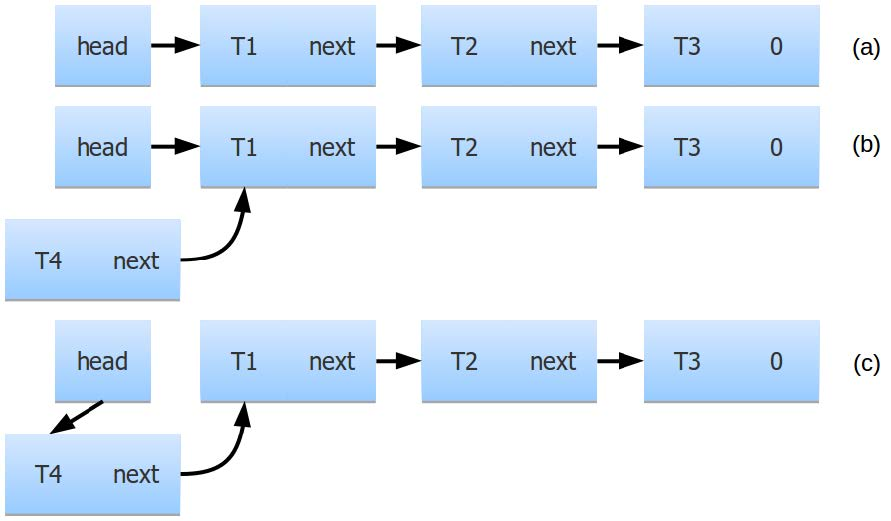
\includegraphics[width=0.9\textwidth]{content/2/chapter7/images/25.jpg}\\
图7.25 - 在单链表的头插入一个新节点
\end{center}

假设我们想在图7.25a所示的列表的头部插入一个新节点。第一步是读取当前头指针,即指向第一个节点的指针。然后用期望值创建新的节点,它的next指针与当前的头指针相同,所以这个节点在当前第一个节点之前链接到链表中(图7.25b)。此时,新节点还不能被任何其他线程访问,因此可以并发地访问数据结构。最后,执行CAS:如果当前头指针没有改变,将用指向新节点的指针替换它(图7.25c)。如果头指针不再具有第一次读取时的值,则读取新值,将其写入新节点的下一个指针,并再次尝试原子CAS。

这是一个简单可靠的算法。这是我们在前一章中看到的发布协议的概括:新数据是在一个线程上创建的,没有考虑线程安全,因为其他线程访问还不能它。作为最后的操作,线程通过原子性地更改可访问所有数据的根指针(我们的例子中是列表的头)来发布数据。如果将新节点插入到另一个节点之后,将自动地更改该节点的next指针。唯一的区别是,多个线程可能试图在同一时间发布新的数据。为了避免数据竞争,我们必须使用\textit{比较和交换}。 

现在,让我们考虑相反的操作,擦除链表的前端节点。这也是通过三个步骤完成的:

%\hspace*{\fill} \\ %插入空行
\begin{center}
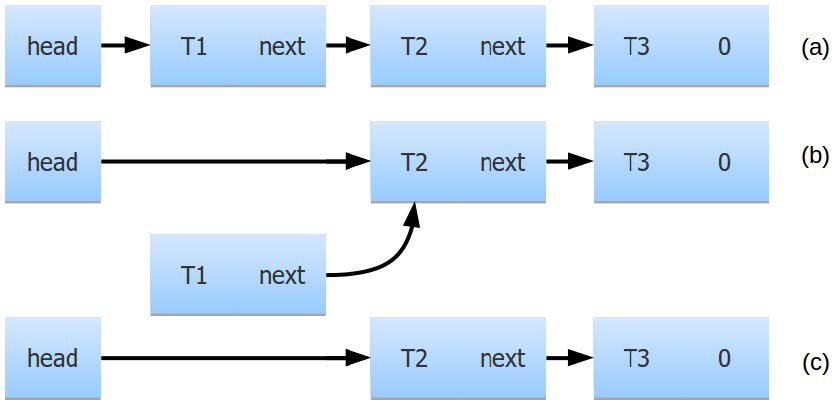
\includegraphics[width=0.9\textwidth]{content/2/chapter7/images/26.jpg}\\
图7.26 - 单链表头部的无锁移除
\end{center}

首先,读取头指针,使用它访问链表的第一个节点,然后读取它的next指针(图7.26a)。然后,我们将next指针的值原子地写入头指针中(图7.26b),但前提是头指针没有改变(CAS)。此时,其他线程访问不能访问前面的第一个节点,这样我们的线程就拥有头指针的原始值,并且可以使用它来删除需要删除的节点(图7.26c)。但是,当我们试图将这两种操作结合起来时,问题就出现了。

让我们假设两个线程同时对链表进行操作,线程A试图删除链表中的第一个节点。第一步是读取头指针和指向next节点的指针,这个指针即将成为列表的新头,但是比较和交换还没有发生。现在,这个头节点是不变的,新头节点是一个值(head'),它只存在于线程A的某个局部变量中。这个时刻如图7.27a所示:

%\hspace*{\fill} \\ %插入空行
\begin{center}
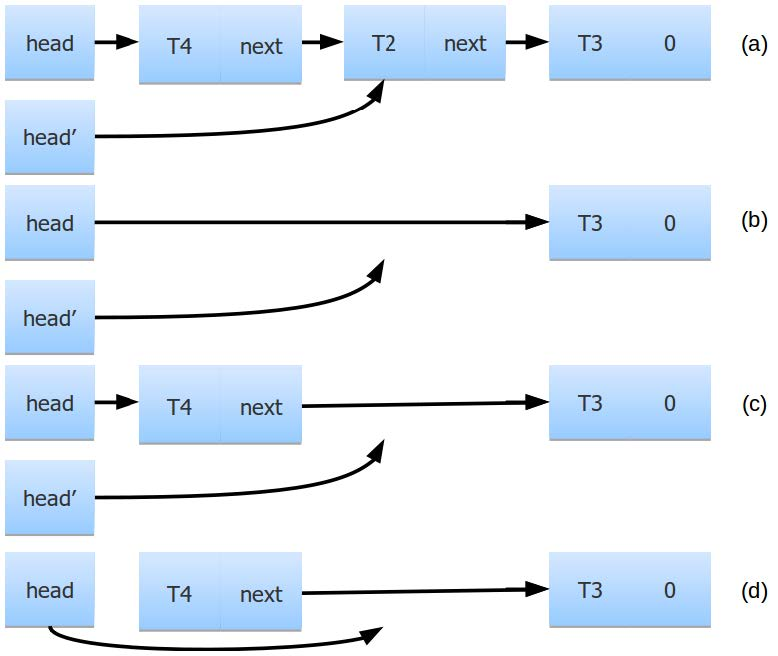
\includegraphics[width=0.9\textwidth]{content/2/chapter7/images/27.jpg}\\
图7.27 - 单链表头部的无锁插入和移除
\end{center}

这时,线程B成功地删除了链表的第一个节点。然后它还会删除下一个节点,使链表保持图7.27b所示的状态(线程A没有取得任何进展)。然后,线程B在链表的开头插入一个新节点(图7.27c)。然而,由于两个已删除节点的内存释放,因此节点T4的新分配重用了之前分配的内存,因此节点T4与原始节点T1拥有了相同的地址。只要删除节点的内存可用于新的分配,这种情况就大概率会发生。事实上,大多数内存分配器更偏爱返回最近释放的内存,前提是它在CPU的缓存中。

现在,线程A终于再次运行了,它要做的操作是比较和交换:如果头指针自线程A上次读取它后没有改变,那么新头成为了现在的头(head')。但是,就线程A所见,头指针的值仍然是相同的(它法观察整个更改历史记录)。CAS操作成功,新的头指针现在指向节点T2以前所使用的内存,而节点T4不再可访问(图7.27d)。自此,整个列表已坏了。

这种故障在无锁数据结构中非常常见,以至于拥有了一个术语:\textbf{A-B-A 问题}。 这里的\textbf{A}和\textbf{B}指的是内存位置:问题是数据结构中的某个指针将其值从A更改为B,然后再返回A。另一个线程只观察初始值和最终值,根本看不到任何更改;比较和交换操作成功,执行的路径是程序员假定数据结构不变的路径。但这个假设是不正确的,数据结构可以任意改变,但没观察到的指针的值的修改,其值就恢复到原来的状态。

问题的根源在于,如果内存回收和分配,那么内存中的指针或地址不能作为数据的唯一标识。这个问题有多种解决方案,但都通过不同的方式完成了相同的事情:必须确保,在读取了一个将会比较-交换使用的指针时,在比较-交换完成之前(成功或不成功),该地址的内存不能释放。如果内存没有释放,那么在同一个地址上就不会发生另一次内存分配,这样就不会出现A-B-A问题。注意,释放内存与删除节点是不一样的。当然,可以使节点不可访问的数据结构的其余部分(删除节点),甚至可以为存储在节点中的数据使用析构函数,但不释放节点所占用的内存。

通过延迟内存回收,出现了许多方法可以用来解决A-B-A问题。如果可能的话,特定于应用程序的选项通常是最简单的。如果知道算法在数据结构的生命周期内不会删除很多节点,那么可以将所有删除的节点存放在一个延迟释放的列表中,以便在删除整个数据结构时删除它们。这种方法的更通用的版本可以描述为应用程序驱动的垃圾收集:所有释放的内存首先放到一个垃圾收集列表中。垃圾内存周期性地返回给主内存分配器,但是在此垃圾收集期间,数据结构上的所有操作都会挂起:正在进行的操作必须在收集开始之前完成,所有新的操作都会阻塞,直到收集完成。这确保了没有比较和交换操作,也可以跨越垃圾收集的间隔。因此,任何操作都不会回收内存。现在流行的RCU(read-copy-update)技术也是这种方法的一种变体。另一种常见的方法是使用风险指针。

本书中,我们将介绍另一种使用原子共享指针的方法(\texttt{std::shared\_ptr}本身不是原子的,但该标准包含了对共享指针进行原子操作所需的必要函数,或者可以为这个特定的应用程序编写自定义函数,使其更快)。让我们重新看一下图7.27b,但是现在所有的指针都是原子共享指针。只要有一个这样的指针指向一个节点,该节点就不能释放。在相同的事件序列中,线程A仍然拥有指向原始节点T1的旧头指针,以及指向节点T2的新头指针head'。

%\hspace*{\fill} \\ %插入空行
\begin{center}
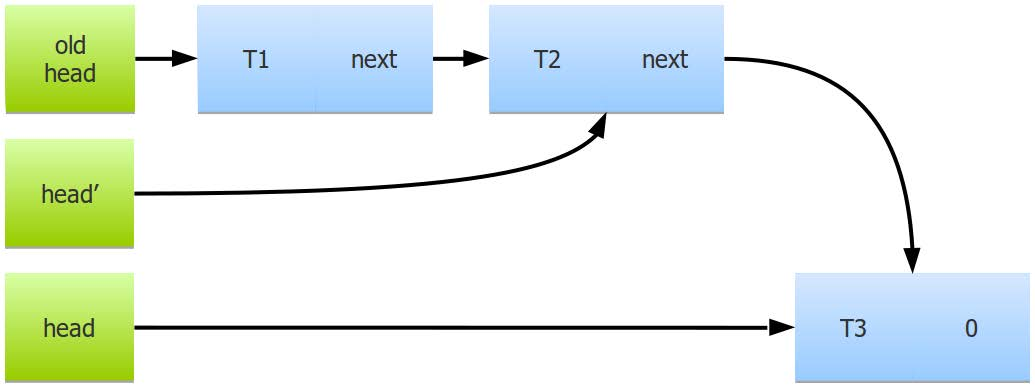
\includegraphics[width=0.9\textwidth]{content/2/chapter7/images/28.jpg}\\
图7.28 - 使用共享指针的单链表头指针——无锁插入和移除
\end{center}

线程B已经从列表中删除了两个节点(图7.28),但是内存还没有释放。不同于当前分配的所有节点的地址,新的节点T4在其他地址上分配。因此,当线程A继续执行时,会发现新的列表头指针与旧的头指针的指向的值不同。比较-交换将失败,线程A将再次尝试操作。此时,将重新读取头指针(并获取节点T3的地址)。因为它是指向节点T1的最后一个共享指针,所以头指针的旧值现在没有了,这个节点因为没有更多的引用而删除了。类似地,只要共享指针head'重置为新的预期值(节点T3的下一个指针),节点T2就会删除。节点T1和T2都没有指向它们的共享指针,因此它们最终也会删除。

当然,这是在节点前插入的情况。为了允许在任何地方插入和删除,必须将所有指向节点的指针转换为共享指针。这包括所有节点的next指针,以及指向链表迭代器中隐藏的节点的指针。这样的设计还有另一个优点:解决了链表遍历(如搜索操作)与插入和删除同时发生的问题。

如果在有指向该列表的迭代器时删除了一个列表节点(图7.29),该节点仍然是已分配的,迭代器有效。即使删除了下一个节点(T3),也不会释放,因为有一个共享指针指向它(节点T2的下一个指针)。迭代器可以遍历整个列表。

%\hspace*{\fill} \\ %插入空行
\begin{center}
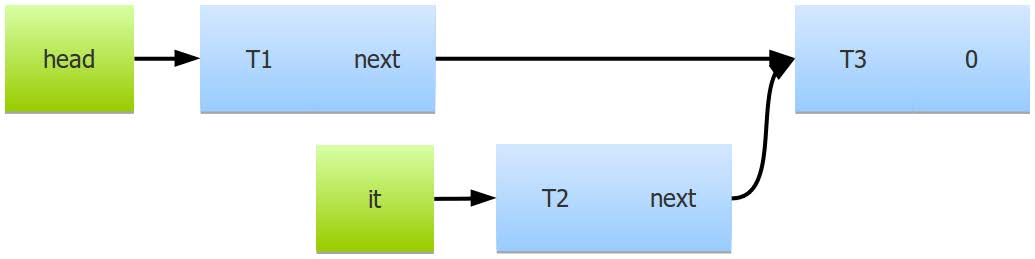
\includegraphics[width=0.9\textwidth]{content/2/chapter7/images/29.jpg}\\
图7.29 - 使用原子共享指针的无锁链表——线程安全的遍历
\end{center}

当然,这个遍历可能包括不再在链表中的节点。也就是说,不需要再从链表的头指针可达的节点开始了。并发数据结构的本质,讨论当前内容没有任何意义。了解链表内容的唯一方法是从列表头遍历到最后一个节点,但当迭代器到达链表末尾时,之前的节点可能已经改变,遍历的结果不再是之前那个“链表”的结果。这种思维方式需要一些时间来适应。

我们不打算展示无锁链表与锁保护链表的基准测试,因为这些基准测试必须基于特定的应用程序。如果只对链表头节点的插入和删除进行基准测试(\texttt{push\_front()}和\texttt{pop\_front()}),那么由自旋锁保护的链表将会更快(原子共享指针并不便宜)。另一方面,如果对同步插入和搜索进行基准测试,则可以使无锁链表的速度最快:遍历包含1M个元素的链表时,锁保护的链表一直处于锁定状态,而无锁列表可以在每个线程上同时进行迭代,同时进行插入和删除操作。无论原子指针有多慢,只要使无锁列表足够长,它就会快。这并不是毫无根据的观察:应用程序可能需要执行一些操作,这些操作需要将链表锁定很长时间,除非能够以某种方式对链表进行分区,以避免死锁。如果需要这样做,那么无锁链表就是目前最快的。如果只需要迭代几个元素,并且从不同时在许多不同的位置,那么用锁保护链表就可以了。

A-B-A问题和解决方案不仅适用于链表,也适用于所有节点数据结构:双链表、树和图。在由多个指针链接的数据结构中,可能会遇到其他问题。首先,即使所有指针都是原子指针,一个接一个地更改两个原子指针也不是一个原子操作。这将导致数据结构中的临时不一致:例如,期望从一个节点到下一个节点,然后返回到前一个节点,这样就回到了原始节点。但在并发性的情况下,这并不总是正确的:如果在这个位置插入或删除节点,其中一个指针可能会在另一个指针之前更新。第二个问题是特定于共享指针或其他使用引用计数的实现:如果数据结构有指针循环,循环中的节点也不会删除,即使没有有外部引用。最简单的例子是双链表,其中两个相邻的节点总是有指向彼此的指针。在单线程程序中,解决这个问题的方法是使用弱指针(在一个双链表中,所有的next指针都可以共享,所有的前一个指针都是弱指针)。这对于并发程序来说不是很好:关键是延迟内存回收,直到没有更多的引用才进行,而弱指针不会这样做。对于这些情况,可能需要额外的垃圾收集机制:在最后一个指向节点的外部指针删除后,必须遍历链接的节点,并检查是否有外部指针指向它们(可以通过检查引用计数来做到),没有外部指针的链表段可以安全删除。对于这类数据结构,可以使用风险指针或显式垃圾收集等替代方法。读者应该参阅有关无锁编程的书籍,以获得关于这些方法的更多信息。

好了,现在就可以结束我们对并行编程高性能数据结构的探索了。现在来总结一下了解到的知识。













